In this measurement, the nucleus used was $^{20}$F.
The decay scheme is given in figure \ref{fig:DecayScheme}.

\begin{figure}[!htb]
	\centerline{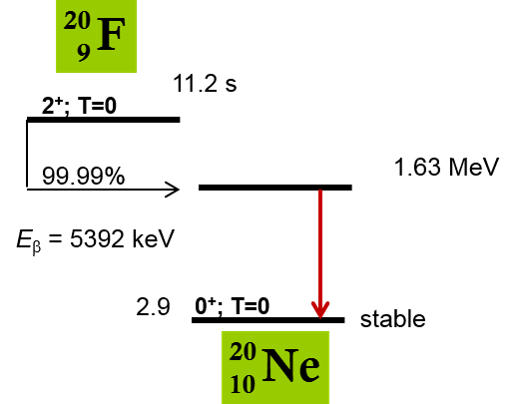
\includegraphics[width=0.78\textwidth]{20FDecayScheme.png}}
	\caption{The decay scheme of $^{20}$F.}
	\label{fig:DecayScheme}
\end{figure}

As seen in the figure, $^{20}$F decays 99.999\% of the time to the first excited state of $^{20}$Ne.
 

\section{Theory Parameters}

For the q-value of the decay, the atomic masses of $^{20}$Ne and $^{20}$F were used.
The decay of $^{20}$F of interest decays to an excited state of the $^{20}$Ne.
The energy of the gamma ray was measured to 0.015 keV \cite{Til98}.

Using the numbers described above and equation \ref{eq:qval}, the q-value for $^{20}$F is 5.901928 (82).
The largest source of uncertainty is in the mass of $^{20}$F.

\begin{equation}
	Q = m_{^{20}F} - (m_{^{20}Na} + E_{\gamma})
	\label{eq:qval}
\end{equation}
